\subsection{User Interface}
\begin{center}
\begin{figure}[h]
	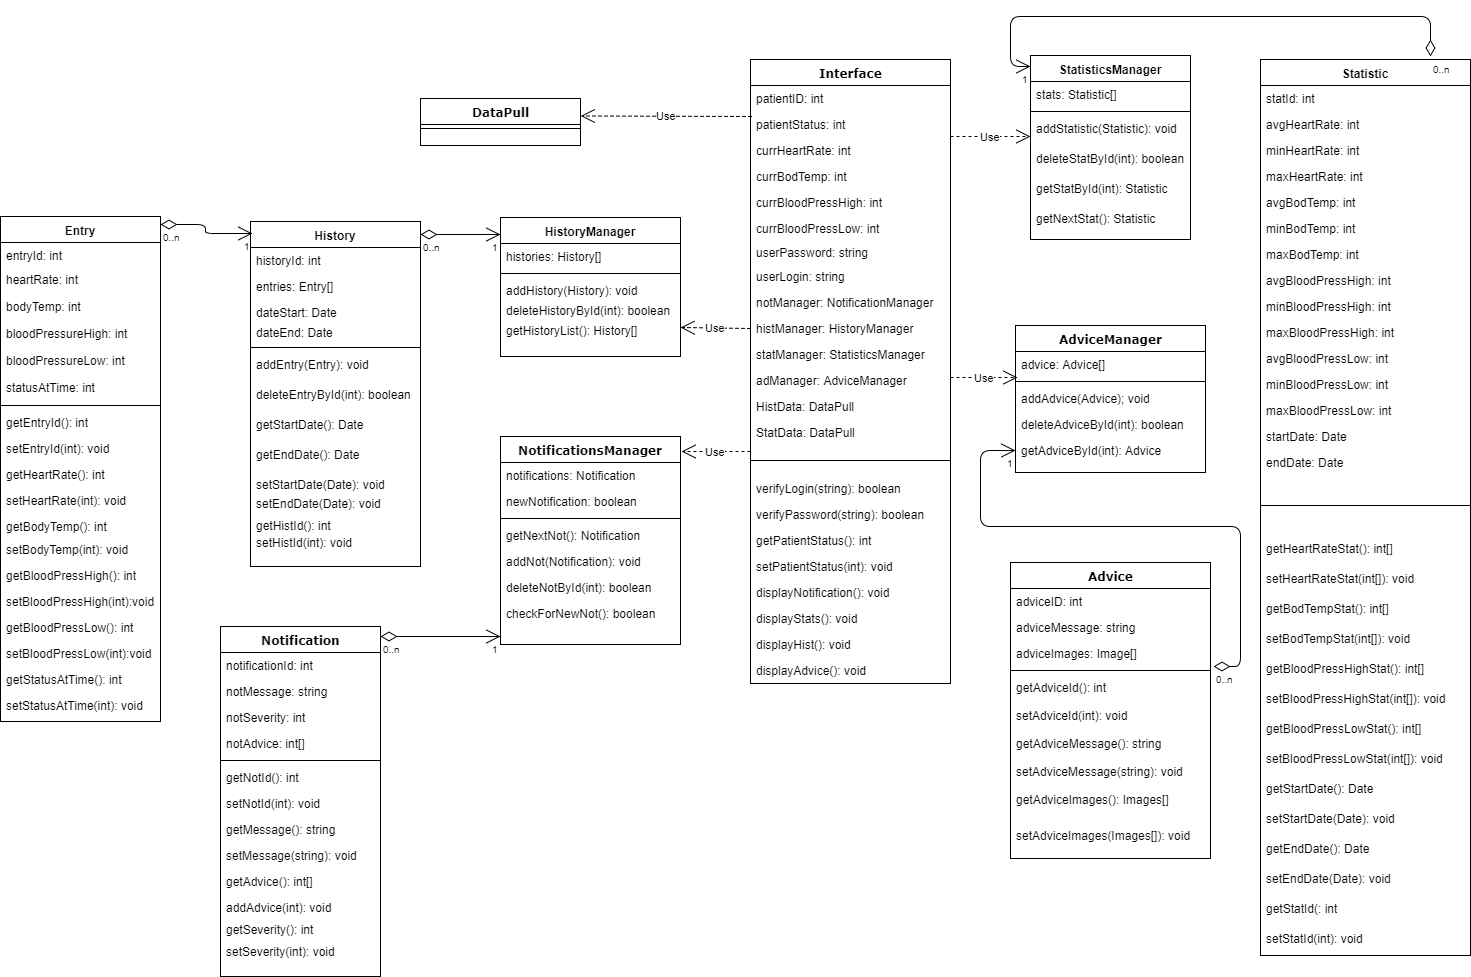
\includegraphics[width=15cm, height=10cm]{Interface.PNG}
\end{figure}
\end{center}

\subsection{Description}
\begin{itemize}
	\item \textbf{DataPull}
	This class is not part of the user interface subsystem but serves to represent where data is recieved from i.e. a module from the server. 
	\item \textbf{Interface}
	This is the main class of the user Interface subsystem. It serves as the reciever of real-time data and the requester of statistical and historical data. It is meant to keep track of user details as well as register new users. It also keeps track and maintains all managers (NotificationsManager, HistoryManager etc...) and displays their content at the users request. It is the main medium of communication between the application and the server, hence its relation with the DataPull class. 
	\item \textbf{StatisticsManager}
	This class acts as a  manager of Statistic class objects. It maintains a list of these objects and provides CRUD (Create, Read, Update, Delete) functionality specifically for statistics. 
	\item \textbf{Statistics}
	This class stores statistical data collected from the server from a specified start and end date. It allows for detailed statistics to be recorded and represented by the interface based on the users selection. This class may be vital in noticing outliers in patient health over a certain period of time. 
	\item \textbf{AdviceManager}
	This is another manager class but for Advice class objects. It also maintains a list and provides CRUD functionality. 
	\item \textbf{Advice}
	This class acts as a container for different advice. Advice is stored in this object in the form of text and is given an ID which is then used to access said advice. Advice may also come with helping images.
  	\item \textbf{HistoryManager}
	This is another manager class but for History class objects. It maintains a list of these objects and provides CRUD functionality. 
  	\item \textbf{History}
	The History class is a special manager class in that it is a manager class of Entry objects but with a specified start and end date, thus it also acts as a data object. It is built in such a way so as to be able to record historical data through the analysis of the collection of Entry objects which it maintains. It provides CRUD functionality for Entry objects. Through using this class, one is able to plot a graph representing the history of the patient's vitals (done by the Interface class). 
  	\item \textbf{Entry}
	Entry is an object class that stores all patient vital's data at a single instance in time. Many Entry objects are used together to establish a history for the patient. 
  	\item \textbf{NotificationsManager}
	This is another manager class but for Notification objects. It maintains a list of Notification objects and provides CRUD functionality. This is also a special case manager class in that it stores Notifications based on alerts from the server and not on request from the user. The Interface class would recieve a real time alert from the server and invoke this class to create and store the appropriate notification to be displayed to the user. User may however delete read notifications or choose to keep them as historical references. 
  	\item \textbf{Notification}
	This class acts as a holder for appropriate alert messages based on real time patient vital values. It stores a status that indicates how critical the alert is as well as an accompanying message describing the alert. It may also store Advice object ID's for reference and instruction for users to use in situations specific to each individual alert.
\end{itemize}
